\documentclass[12pt]{article}
\usepackage{graphicx}
\usepackage{subcaption}
\usepackage{hyperref}
\usepackage{float}
\usepackage{mathtools}

\title{CMSC 6950 Project}
\date{June 2021}
\author{Kabir Zubaer} 

\setlength\parindent{0pt}
\begin{document}
\maketitle
\section{Introduction}

The ocean is a key component of the Earth’s climate system. It therefore needs continuous
real-time monitoring to help scientists better understand its dynamics and to predict its evolution. All around the world, oceanographers have managed to join their efforts and set up a
Global Ocean Observing System among which Argo is a key component.

Argo is a global network of nearly 4000 autonomous probes measuring pressure, temperature
and salinity from the surface to 2000m depth every 10 days. The localisation of these probes
is nearly random between the 60o parallels (see live coverage here). Data from the probes
are collected by satellite in real-time, processed by several data centers, merged in a single
dataset (comprising of more than 2.3 million vertical profiles as of June 2020) and made freely
available to anyone through an ftp server or monthly zip snapshots.

\section{Results}

Herein, the results for each computational task will be presented. The first computational task will focus on visualizing the position of Argo floats in a region Oceania,  and how the total number of floats changes each year. The second computational task is used to visualize the trajectory and temperature variation of two Argo floats with time since the float's deployment.
  
\subsection{Task 1- Total Argo float numbers through time}

The aim of my first computational task = to retrieve Argo float data collected from June 2015 to December 2015 using argopy and then use this data to visualize the change in the total number of Argo floats per month within a region of the Oceania.  

\begin{figure}[H]
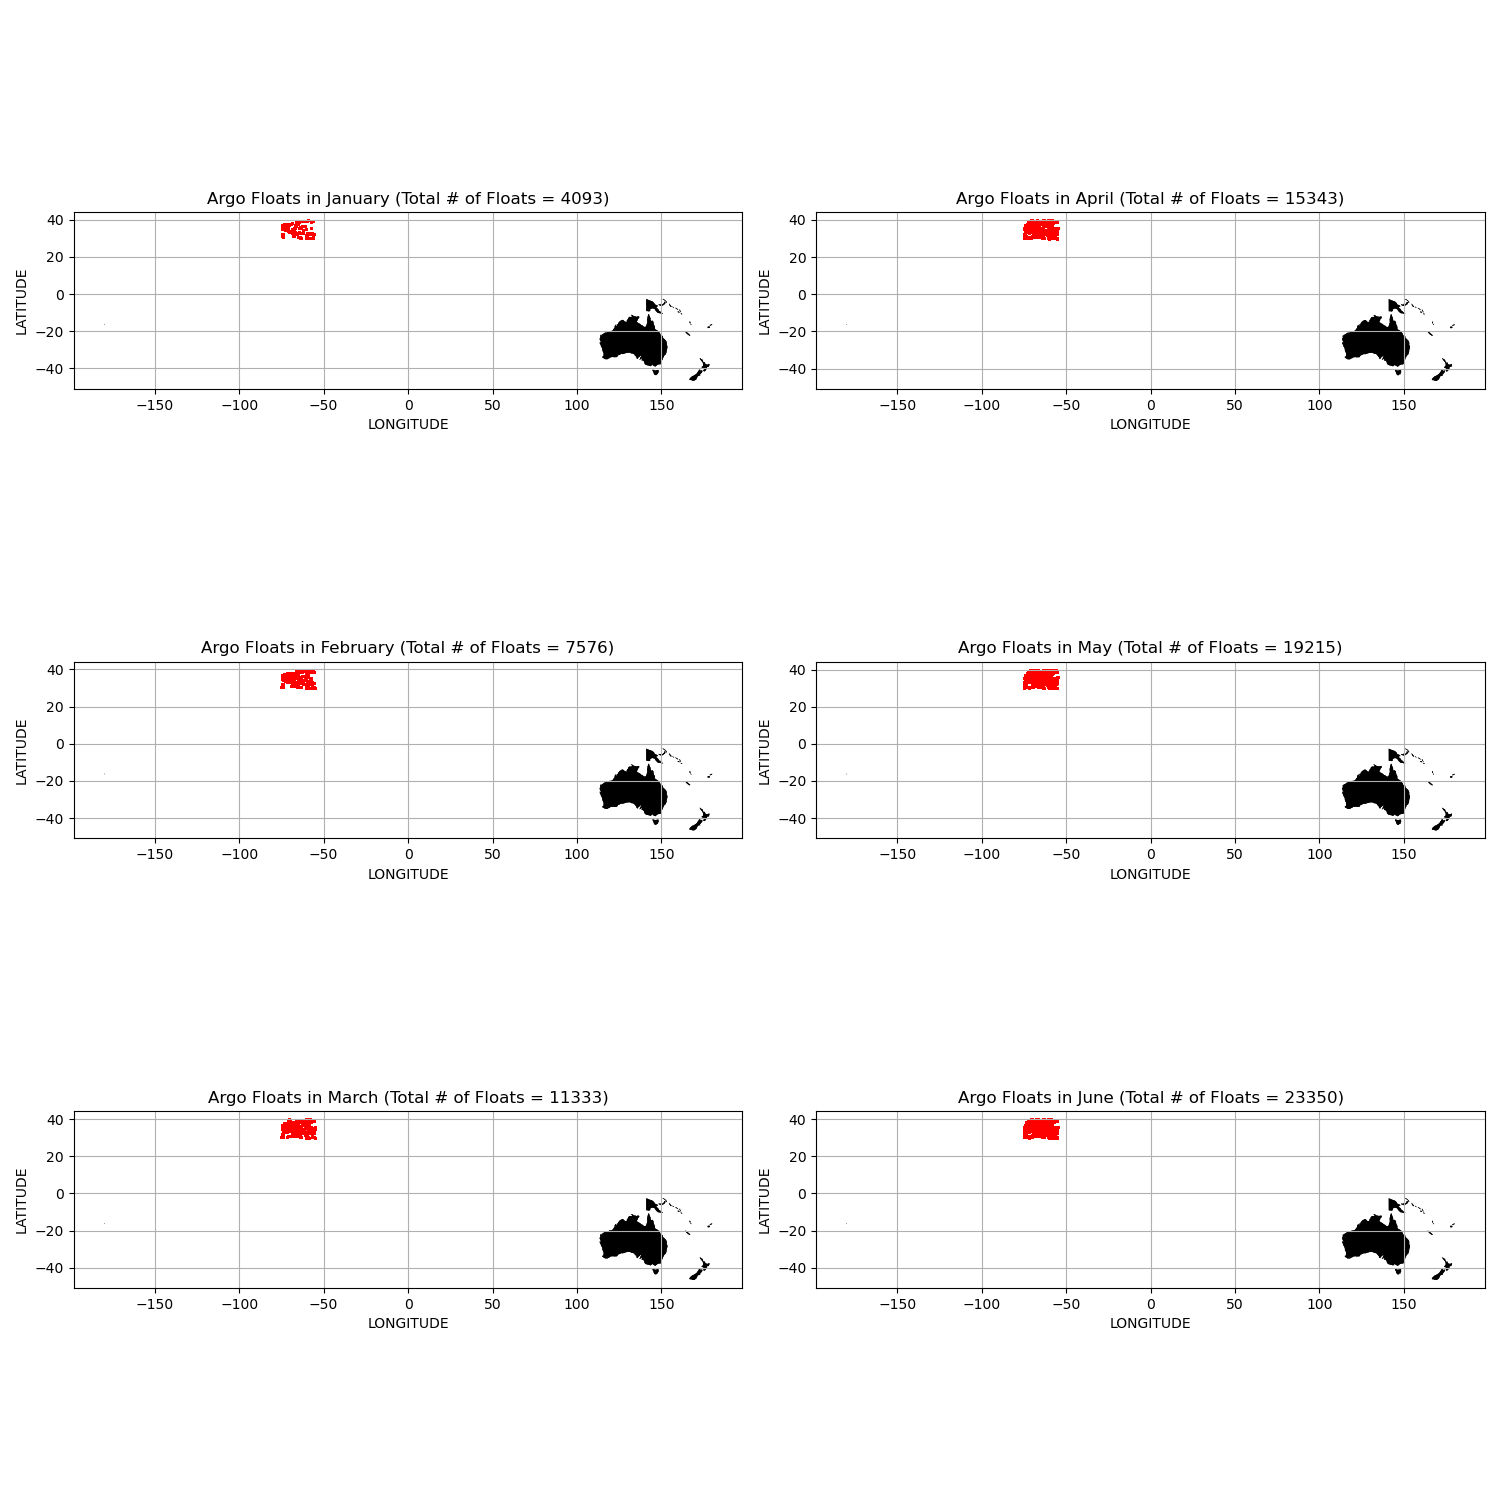
\includegraphics[width=\textwidth,height=\textheight,keepaspectratio]{monthly.png}
\caption{Total number of Argo floats for each month from June 2015 to December 2015  in a region Oceania.}
\label{fig:task 1}
 
\end{figure}




\subsection{Task 2 - Showing Level, Pressure, Salinity, and Temperature through time.}

In this task I try to find out Level, Pressure, Salinity, and Temperature for each month from June 2015 to December 2015  in a region Oceania

\begin{figure}[H]
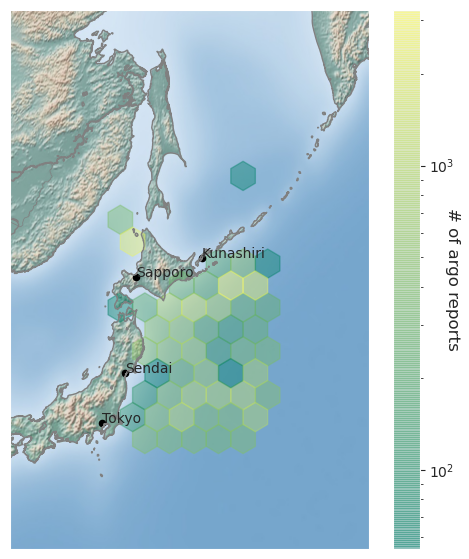
\includegraphics[width=\textwidth,height=\textheight,keepaspectratio]{locations.png}
\caption{Hexbin of Argo floats for each month from June 2015 to December 2015  in a region Oceania.}
\label{fig:task 2}
 
\end{figure}

\section{Conclusion}
In this task, I try to solve two computational tasks involving argopy, I have fetched data from external sources for the period of six months. In case of ploting and visualization I used different python library.

\end{document}